% !TeX root = Microwave.tex
\chapter{Transmission Line Theory 传输线理论 }
\section{Transmission Line Equation 传输线方程 }

% \paragraph{Plane Waves in a Lossless Medium}
% ~\\[-15pt]


% In a lossless medium, $\varepsilon,\,\mu\in\mathfrak{R}$, and so $k$ is real.

\subsection{微波传输线}
    良导体的集肤效应:
    \begin{equation}
        \alpha=\sqrt{\frac{\omega\mu\sigma}{2}}=\frac{1}{\delta}
    \end{equation}

    where $\alpha$ is the \emph{attenuation constant} and $\delta$ is the \emph{skin depth}.

\subsection{传输线方程}
    微波传输线的四参数模型:
    \begin{subequations}
        \begin{numcases}{}
        -\frac{\partial u}{\partial z}=Ri+L \frac{\partial i}{\partial t}\\
        -\frac{\partial i}{\partial z}=Gu+C \frac{\partial u}{\partial t}
        \end{numcases}
    \end{subequations}
    对于时谐场:
    \begin{subequations}
        \begin{numcases}{}
        -\frac{\mathrm{d}u}{\mathrm{d}z}=i(R+\mathrm{j}\omega L)=Zi\\
        -\frac{\mathrm{d}i}{\mathrm{d}z}=u(G+\mathrm{j}\omega C)=Yu
        \end{numcases}
    \end{subequations}
    特别注意,这里的$R,\,Z$单位为\si{\ohm\per\metre},$G,\,Y$的单位为\si{\siemens\per\metre}。


\subsection{无耗传输线方程}
    无耗$\Rightarrow R=G=0$(导线上没有电阻或电纳)
    \begin{subequations}
        \begin{numcases}{}
        -\frac{\mathrm{d}u}{\mathrm{d}z}=\mathrm{j}\omega Li \label{Equ: Lossless Medium dudz}\\
        -\frac{\mathrm{d}i}{\mathrm{d}z}=\mathrm{j}\omega Cu \label{Equ: Lossless Medium didz}
        \end{numcases}
    \end{subequations}
    将式 (\ref{Equ: Lossless Medium dudz})代入式 (\ref{Equ: Lossless Medium didz})或者反之,可以解得:
    \begin{subequations}
        \begin{numcases}{}
        \frac{\mathrm{d}^2u}{\mathrm{d}z^2}+\beta^2u=0 \label{Equ: Lossless Transmission d2udz2}\\
        \frac{\mathrm{d}^2i}{\mathrm{d}z^2}+\beta^2i=0 \label{Equ: Lossless Transmission d2idz2}
        \end{numcases}
    \end{subequations}
    其中$\beta=\omega\sqrt{LC}$为相位常数。
    解此二阶微分方程,得:
    \begin{subequations}
        \begin{numcases}{}
        u(z)=A_1 \mathrm{e}^{-\mathrm{j}\beta z}+A_2 \mathrm{e}^{\mathrm{j}\beta z}\label{Equ: Lossless Transmission u(z)}\\
        i(z)=\frac{1}{Z_0}\left(A_1 \mathrm{e}^{-\mathrm{j}\beta z} {\color{red}\,-\,} A_2 \mathrm{e}^{\mathrm{j}\beta z}\right)\label{Equ: Lossless Transmission i(z)}
        \end{numcases}
    \end{subequations}
    其中,$Z_0=\sqrt{\frac{L}{C}}$为特性阻抗,单位为\si{\ohm}。确定$A_1,\,A_2$还需边界条件。

    \paragraph{本征模思想:}任何传输线上的电压是入射波和反射波的叠加,其形式确定如式(\ref{Equ: Eigenmode u=(u+)+(u-)}),不同传输线的区别仅在与入射波和反射波的成分不同。
    \begin{subequations}\label{Equ: Eigenmode u(z) and i(z)}
        \begin{numcases}{}
            u(z)=u^+_0 \mathrm{e}^{-\mathrm{j}\beta z}+u^-_0 \mathrm{e}^{\mathrm{j}\beta z}\label{Equ: Eigenmode u=(u+)+(u-)}\\
            i(z)=\frac{u^+_0}{Z_0} \mathrm{e}^{-\mathrm{j}\beta z} {\color{red}\,-\,} \frac{u^-_0}{Z_0} \mathrm{e}^{\mathrm{j}\beta z}
        \end{numcases}
    \end{subequations}

\subsection{无耗传输线的边界条件}\label{Sec: Boundary conditions of lossless transmission lines}
    以源端为原点建立$z$轴,正方向为负载方向。以终端为原点建立$z'$轴,正方向为电源方向。


    设导线长度为$l$,则导线上源端坐标系下坐标为$z=z_0$的点,在另一个坐标系下表示为$z'=l-z_0$。

    \begin{enumerate}
        \item {\bfseries 终端边界条件:}已知负载上的电压$U_l$、电流$I_l$
            \begin{equation}
                \begin{bmatrix}
                    u(z')\\
                    i(z')
                \end{bmatrix}
                =
                \begin{bmatrix}
                    \cos{\beta z'}&\mathrm{j}Z_0\sin{\beta z'}\\
                    \mathrm{j}\frac{1}{Z_0}\sin{\beta z'}&\cos{\beta z'}
                \end{bmatrix}
                \begin{bmatrix}
                    u(l)\\
                    i(l)
                \end{bmatrix}\label{Equ: u(z'), i(z')|u(l), i(l)}
            \end{equation}
            其中,$z'=l-z$。虽然这种用A参数矩阵描述的二端口网络形式很好记,但有时还会用到它的本征模形式:
            \begin{subequations}
                \begin{numcases}{}
                    u(z)=\frac{1}{2}(U_l+Z_0I_l)\mathrm{e}^{\mathrm{j}\beta l} \,\mathrm{e}^{-\mathrm{j}\beta z}+\frac{1}{2}(U_l-Z_0I_l)\mathrm{e}^{-\mathrm{j}\beta l}\, \mathrm{e}^{\mathrm{j}\beta z}\\
                    i(z)=\frac{1}{2Z_0}(U_l+Z_0I_l)\mathrm{e}^{\mathrm{j}\beta l}\, \mathrm{e}^{-\mathrm{j}\beta z} {\color{red}\,-\,} \frac{1}{2Z_0}(U_l-Z_0I_l)\mathrm{e}^{-\mathrm{j}\beta l}\, \mathrm{e}^{\mathrm{j}\beta z}
                \end{numcases}
            \end{subequations}
            或$z'$下
            \begin{subequations}\label{Equ: 无耗传输线终端边界条件电压电流表达式z'}
                \begin{numcases}{}
                    u(z')=\frac{1}{2}(U_l+Z_0I_l)\mathrm{e}^{\mathrm{j}\beta z'} +\frac{1}{2}(U_l-Z_0I_l)\mathrm{e}^{-\mathrm{j}\beta z'}\\
                    i(z')=\frac{1}{2Z_0}(U_l+Z_0I_l)\mathrm{e}^{\mathrm{j}\beta z'} {\color{red}\,-\,} \frac{1}{2Z_0}(U_l-Z_0I_l)\mathrm{e}^{-\mathrm{j}\beta z'}
                \end{numcases}
            \end{subequations}
        \item {\bfseries 源端边界条件:}已知源端处双导线之间电压$U_0$、电流$I_0$
            \begin{equation}
                \begin{bmatrix}
                    u(z)\\
                    i(z)
                \end{bmatrix}
                =
                \begin{bmatrix}
                    \cos{\beta z}&-\mathrm{j}Z_0\sin{\beta z}\\
                    -\mathrm{j}\frac{1}{Z_0}\sin{\beta z}&\cos{\beta z}
                \end{bmatrix}
                \begin{bmatrix}
                    u(0)\\
                    i(0)
                \end{bmatrix}\label{Equ: u(z), i(z)|u(0), i(0)}
            \end{equation}
            它的本征模形式为:
            \begin{subequations}
                \begin{numcases}{}
                    u(z)=\frac{1}{2}(U_0+Z_0I_0) \mathrm{e}^{-\mathrm{j}\beta z}+\frac{1}{2}(U_0-Z_0I_0) \mathrm{e}^{\mathrm{j}\beta z}\\
                    i(z)=\frac{1}{2Z_0}(U_0+Z_0I_0) \mathrm{e}^{-\mathrm{j}\beta z} {\color{red}\,-\,} \frac{1}{2Z_0}(U_0-Z_0I_0) \mathrm{e}^{\mathrm{j}\beta z}
                \end{numcases}
            \end{subequations}
        \item {\bfseries 电源、阻抗条件:}已知电源电压$E_g$、内阻$Z_g$,负载$Z_l$


            定义{\color{orange} 电源反射系数}和{\color{orange} 负载反射系数}:
            \begin{align}
                \varGamma_g&=\frac{Z_g-Z_0}{Z_g+Z_0}\\
                \varGamma_l&=\frac{Z_l-Z_0}{Z_l+Z_0}
            \end{align}
            $\varGamma_g$反映了电源阻抗与特征阻抗的匹配程度,即体现了电源吸收反射波能力的大小。
            $\varGamma_l$反应了负载与特征阻抗的匹配程度,不匹配的负载是反射波的源。


            {\color{red}NOTE:} 在稳态下只有$\varGamma_l$起作用,当$\varGamma_l=0$时,$\varGamma_g$没有意义。

            \begin{numcases}{}
                \mbox{源端:}u(0)=E_g-i(0)Z_g\xlongequal{i(0)=\frac{1}{Z_0}(A_1-A_2)}E_g-\frac{Z_g}{Z_0}(A_1-A_2)=A_1+A_2\notag\\
                \mbox{终端:}u(l)=i(l)Z_l\xlongequal{i(l)=\frac{1}{Z_0}(A_1 \mathrm{e}^{-\mathrm{j}\beta l}-A_2 \mathrm{e}^{\mathrm{j}\beta l})}Z_l\frac{1}{Z_0}(A_1 \mathrm{e}^{-\mathrm{j}\beta l}-A_2 \mathrm{e}^{\mathrm{j}\beta l})=A_1 \mathrm{e}^{-\mathrm{j}\beta l}+A_2 \mathrm{e}^{\mathrm{j}\beta l}\notag
            \end{numcases}

            由此得到关于$A_1,A_2$的方程组,使用\emph{Cramer's Rule}解出$A_1,A_2$,代入式(\ref{Equ: Lossless Transmission u(z)})和式(\ref{Equ: Lossless Transmission i(z)})得:
            \begin{subequations}
                \begin{numcases}{}
                    u(z)=\frac{E_gZ_0}{(Z_g+Z_0)(1-\varGamma_g\varGamma_l \mathrm{e}^{-\mathrm{j}2\beta l})}\left( \mathrm{e}^{-\mathrm{j}\beta z} + \varGamma_l \mathrm{e}^{-\mathrm{j}2\beta l} \mathrm{e}^{\mathrm{j}\beta z}\right)\label{Equ: u(z)|E_g, Z_h, Z_l}\\
                    i(z)=\frac{E_g}{(Z_g+Z_0)(1-\varGamma_g\varGamma_l \mathrm{e}^{-\mathrm{j}2\beta l})}\left( \mathrm{e}^{-\mathrm{j}\beta z} {\color{red}\,-\,} \varGamma_l \mathrm{e}^{-\mathrm{j}2\beta l} \mathrm{e}^{\mathrm{j}\beta z}\right)\label{Equ: i(z)|E_g, Z_h, Z_l}
                \end{numcases}
            \end{subequations}
        \end{enumerate}


\section{Transmission Analysis \Rmnum{1} 传输状态分析 \Rmnum{1} }

\begin{table}[ht]
    \setlength{\belowrulesep}{-5mm} %在线条[不包括\bottomrule]下面增加一段垂直距离
    \setlength{\aboverulesep}{-5mm} %在线条[不包括\toprule]上面增加一段垂直距离
    \centering
    \resizebox{\textwidth}{!}
    {
    \begin{tabular}{c}
        \toprule
        \hspace{15cm}~\\
        \hline
    \end{tabular}
    }
    \textbf{传输线的三个工作参数:反射系数、输入阻抗、驻波比}
    \resizebox{\textwidth}{!}
    {
    \begin{tabular}{c}
        \hline
        \hspace{15cm}~\\
        \bottomrule
    \end{tabular}
    }
\end{table}

\subsection{任意位置的反射系数}
    \subsubsection{反射系数$\varGamma(z)$}
    通常所说的反射系数,指的是从负载方向反射回电源方向的电压反射系数,常定义在$z'$坐标系下,记作$\varGamma(z')$
    \begin{equation}
        \varGamma(z')=\frac{u^-(z')}{u^+(z')}=\frac{u^-_l \mathrm{e}^{-\mathrm{j}\beta z'}}{u^+_l \mathrm{e}^{\mathrm{j}\beta z'}}=\varGamma_l \mathrm{e}^{-\mathrm{j}2\beta z'}\label{Equ: Reflection Coefficient at z'}
    \end{equation}
    \begin{center}
        $\varGamma(z'=l)$是否等于$\varGamma_g$? ——  {\color{red} 否。它们是完全独立的}
    \end{center}
    其中$u^+_l$即将$z=l$代入章节\ref{Sec: Boundary conditions of lossless transmission lines}中的本征模电压表达式,但只取向$z+$方向(也即$z'-$方向)传播的分量;同理,$u^-_l$即负载处向$z-$方向(也即$z'$方向)的电压分量。{\color{gray}可以利用第三种边界条件来验证一下, $u^+_l,\, u^-_l$分别为:
    \begin{subequations}
        \begin{numcases}{}
            u^+_l=u^+(z=l)=u^+(z'=0)=\frac{E_gZ_0 \mathrm{e}^{-\mathrm{j}\beta l}}{(Z_g+Z_0)(1-\varGamma_g\varGamma_l \mathrm{e}^{-\mathrm{j}2\beta l})}\\
            u^-_l=u^-(z=l)=u^-(z'=0)=\frac{E_gZ_0 \varGamma_l\mathrm{e}^{-\mathrm{j}\beta l}}{(Z_g+Z_0)(1-\varGamma_g\varGamma_l \mathrm{e}^{-\mathrm{j}2\beta l})}
        \end{numcases}
    \end{subequations}
    可见它们的确满足$u^-_l=\varGamma_l u^+_l$
    }
    \paragraph{电流反射系数:}
    \begin{equation}
        \varGamma_I(z')=\frac{i^-(z')}{i^+(z')}=\frac{i^-_l \mathrm{e}^{-\mathrm{j}\beta z'}}{i^+_l \mathrm{e}^{\mathrm{j}\beta z'}}{\color{red}\,=\frac{-u^-(z')/Z_0}{u^+(z')/Z_0}=-\varGamma(z')}\label{Equ: Reflection Coefficient of current at z'}
    \end{equation}
    \paragraph{使用前向电压电流和反射系数表示任意位置的电压电流:}(称$z+$方向为前向)
    ~\\[-15pt]

    根据\hyperref[Equ: Reflection Coefficient at z']{式(\ref*{Equ: Reflection Coefficient at z'})}和\hyperref[Equ: Reflection Coefficient of current at z']{式(\ref*{Equ: Reflection Coefficient of current at z'})},将入射波与反射波相加:
    \begin{subequations}\label{Equ: 电压或电流波的叠加}
        \begin{numcases}{}
            u(z')=u^+(z')\left[1+\varGamma(z')\right]=u^+_l(1+\varGamma_l \mathrm{e}^{-\mathrm{j}2\beta z'})\mathrm{e}^{\mathrm{j}\beta z'}\\
            i(z')=i^+(z')\left[1-\varGamma(z')\right]=i^+_l(1-\varGamma_l \mathrm{e}^{-\mathrm{j}2\beta z'})\mathrm{e}^{\mathrm{j}\beta z'}
        \end{numcases}
    \end{subequations}

    \paragraph{输入阻抗与特征阻抗通过反射系数转化:}
    ~\\[-15pt]

    上式所示的方程组上下相除可以得到任意位置输入阻抗$Z(z')$和传输线特征阻抗$Z_0$的关系:
    \begin{equation}
        Z(z')=Z_0\frac{1+\varGamma(z')}{1-\varGamma(z')}\label{Equ: Z(z')<-->Z_0}
    \end{equation}

    \begin{boxedminipage}{\textwidth}
        \vspace{5pt}
        注意各种阻抗的区别和关系:
        \begin{equation*}
        \mbox{}
        \begin{cases}
                \mbox{输入阻抗:}\mbox{(入射反射叠加)电压波与(入射反射叠加)电流波的比值} \\
                \mbox{特性阻抗:}\mbox{ 前向电压波与前向电流波的比值;或后向电压波与后向电流波的比值的相反数} \\
                \mbox{波阻抗:} \mbox{前向电场与前向磁场的比值}
        \end{cases}
        \end{equation*}
    \end{boxedminipage}


    \paragraph{反射系数的性质:}
    \begin{enumerate}
        \item 无耗传输系统中,\underline{反射系数的模值处处相等$|\varGamma(z')|=|\varGamma_l|$},辐角与移动的距离成正比;
        \item 反射系数呈周期性,关于电长度$\theta$的周期为$\pi$,关于$z'$的周期为$\frac{\lambda_g}{2}=\frac{\pi}{\beta}$。
        \item 反射系数模值不大于1(可从能量守恒的角度理解)。
    \end{enumerate}

\subsection{任意位置的输入阻抗}
    \subsubsection{输入阻抗$Z(z)$}
    输入阻抗是一个宏观参数,并不是只和入射波有关,而是导线在\underline{稳态下}的电压与流过此处的电流之比。在$z'$坐标系中,任一点的输入阻抗为:
    \begin{equation}
        Z(z')=\frac{u(z')}{i(z')}
            \xlongequal[\mbox{\scriptsize(终端边界条件)}]{\mbox{式(\ref{Equ: u(z'), i(z')|u(l), i(l)})}}
        \frac{U_l\cos{\beta z'}+\mathrm{j}Z_0I_l\sin{\beta z'}}{\mathrm{j}\frac{1}{Z_0}U_l\sin{\beta z'}+I_l\cos{\beta z'}}
            \xlongequal[\mbox{\scriptsize(同除$I_l\cos{\beta z'}$)}]{Z_l=\frac{U_l}{I_l}}
        \frac{\frac{Z_l}{Z_0}+\mathrm{j}\tan{\beta z'}}{\mathrm{j}\frac{Z_l}{Z_0}\tan{\beta z'}+1}
    \end{equation}
    该式也可以由\hyperref[Equ: Z(z')<-->Z_0]{式(\ref*{Equ: Z(z')<-->Z_0})} 代入$\varGamma_l$得到:
    \begin{align}
        Z(z')&=Z_0\frac{1+\varGamma_l \mathrm{e}^{-\mathrm{j}2\beta z'}}{1- \varGamma_l \mathrm{e}^{-\mathrm{j}2\beta z'}}
        % \xlongequal[\mbox{同乘$(Z_l+Z_0)$}]{\mbox{同乘$\mathrm{e}^{\mathrm{j}\beta z'}$}}
        \quad\mbox{(上下同乘$(Z_l+Z_0)\mathrm{e}^{\mathrm{j}\beta z'}$)}\notag\\
        &=Z_0\frac{(Z_l+Z_0)(\cos\beta z'+\mathrm{j}\sin\beta z')+(Z_l-Z_0)(\cos\beta z'-\mathrm{j}\sin\beta z')}
            {(Z_l+Z_0)(\cos\beta z'+\mathrm{j}\sin\beta z')-(Z_l-Z_0)(\cos\beta z'-\mathrm{j}\sin\beta z')}\notag\\
        &=Z_0\frac{2Z_l\cos\beta z'+2Z_0 \mathrm{j}\sin\beta z'}{2Z_l \mathrm{j}\sin\beta z'+2Z_0 \cos\beta z'}
            \quad\mbox{(上下同除以$2\cos\beta z'$)}\notag\\
        &=Z_0\frac{Z_l+Z_0 \mathrm{j}\tan\beta z'}{Z_l \mathrm{j}\tan\beta z'+Z_0}\label{Equ: 使用终端反射系数表示输入阻抗}
    \end{align}

    \paragraph{输入阻抗的性质:}

    \begin{enumerate}
        \item 通过控制传输长度,微波传输线对输入阻抗具有阻抗变换作用;


        常利用电长度$\theta=\beta z$取值为$m\pi+\frac{\pi}{2}$(即距离$(\frac{1}{2}m+\frac{1}{4})\lambda_g$)来实现阻抗的反演变换:
        \begin{align*}
            Z(z'\pm\frac{1}{4}\lambda_g)
            &=Z_0\frac{1+\varGamma_l \mathrm{e}^{(-\mathrm{j}2\beta z'\mp\mathrm{j}\pi)}}{1- \varGamma_l \mathrm{e}^{(-\mathrm{j}2\beta z'\mp\mathrm{j}\pi)}}\\
            &=Z_0\frac{1-\varGamma_l \mathrm{e}^{-\mathrm{j}2\beta z'}}{1+\varGamma_l \mathrm{e}^{-\mathrm{j}2\beta z'}}\\
            &=Z_0^2 \frac{1}{Z_0\frac{1+\varGamma_l \mathrm{e}^{-\mathrm{j}2\beta z'}}{1-\varGamma_l \mathrm{e}^{-\mathrm{j}2\beta z'}}}\\
            &=\frac{Z_0^2}{Z(z')}\doteq Z_0^2Y(z')
        \end{align*}
        \item 输入阻抗呈周期性,与反射系数的周期相同。

    \end{enumerate}

    \paragraph{总结:}任意位置的反射系数和输入阻抗及其转换关系
    \begin{figure}[htp]
        \centering
        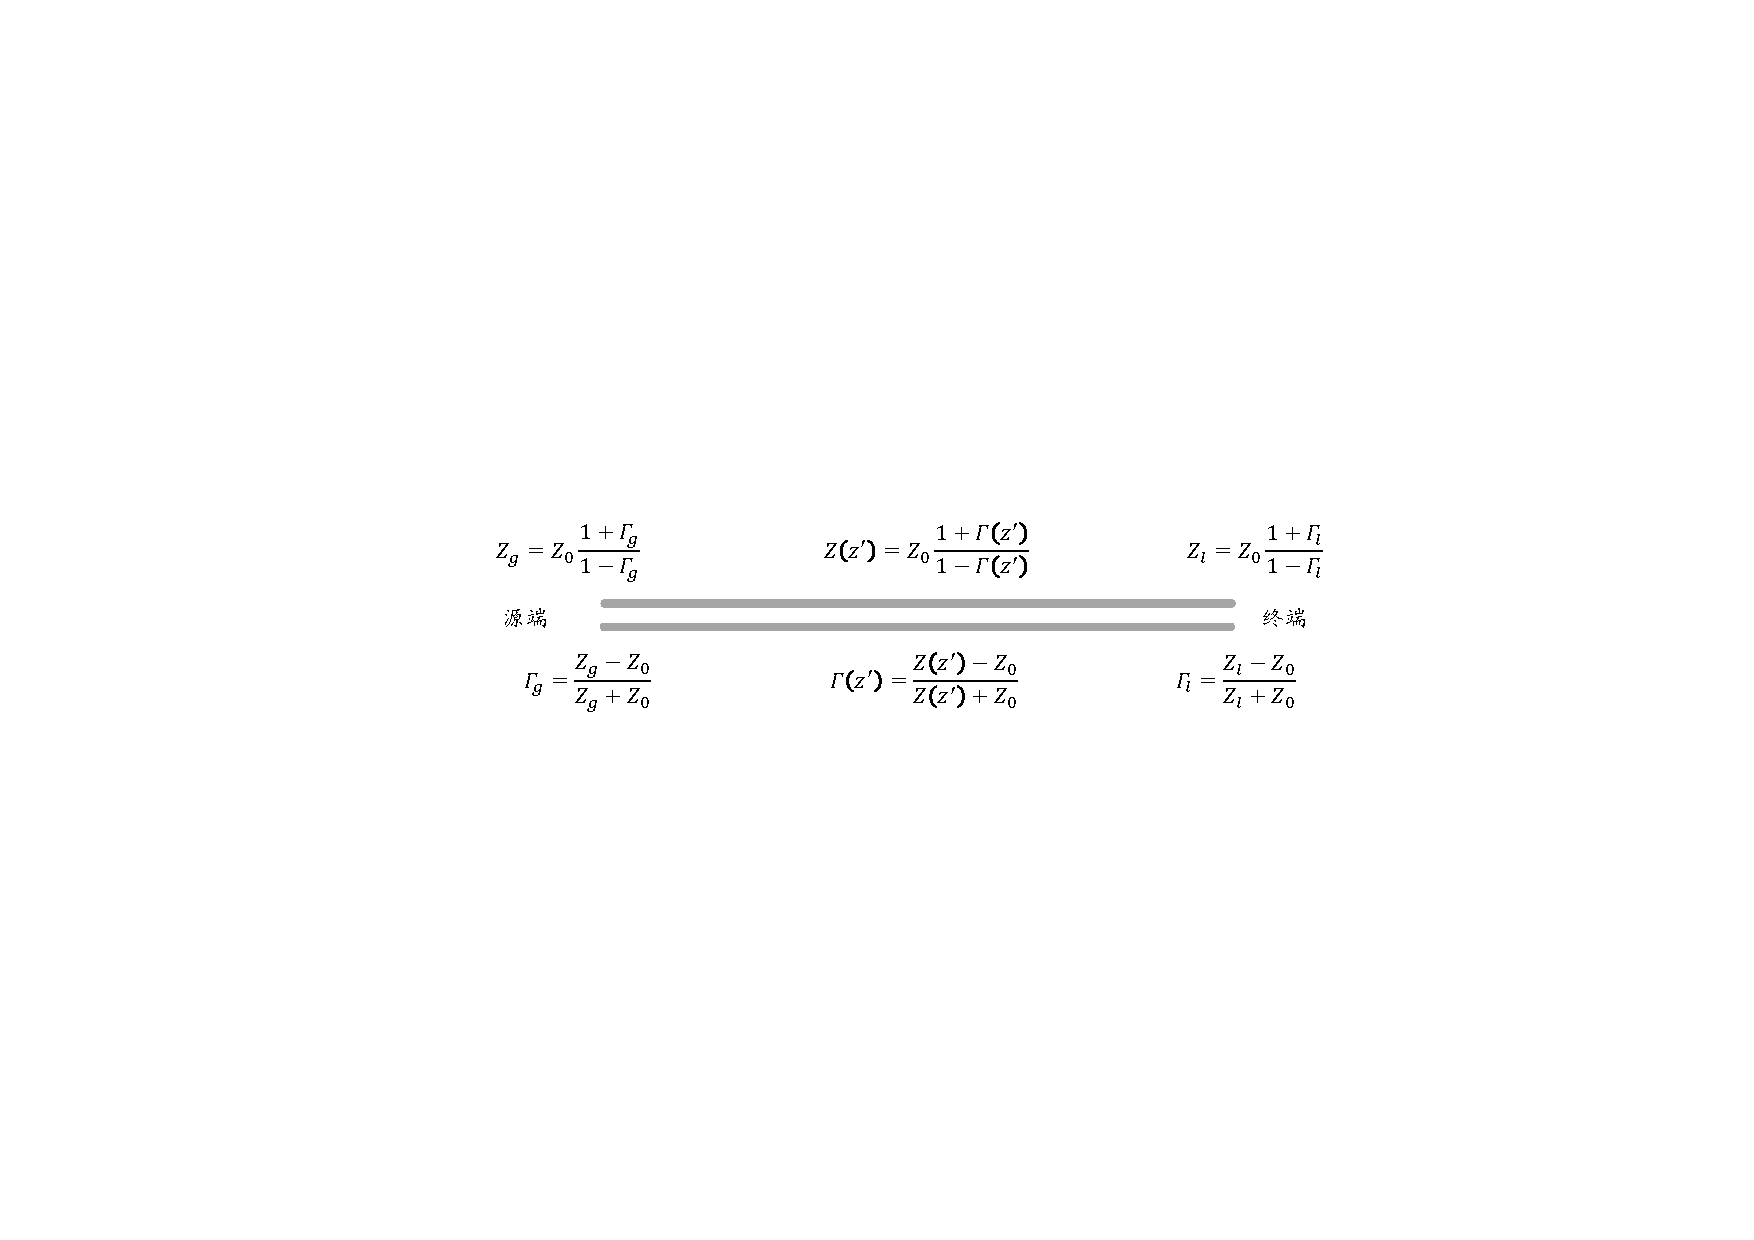
\includegraphics[width=14cm]{figure/1-1.pdf}
    \end{figure}

\subsection{电压驻波比——传输系统的不变量}
    电压驻波比(Voltage Standing Wave Ratio)\emph{abbr.} VSWR,也称驻波比(\emph{abbr.} SWR),定义为:
    \begin{equation}
        \rho=\frac{1+\left\vert\varGamma_l\right\vert}{1-\left\vert\varGamma_l\right\vert}\in[1,\infty)
    \end{equation}
    对于一个确定的传输系统,由于负载确定,所以$\varGamma_l$的模值确定,因此$\rho$是定值。


    根据 \hyperref[Equ: 电压或电流波的叠加]{式(\ref*{Equ: 电压或电流波的叠加})} ,电压或电流的叠加波振幅的极值只会在$\mathrm{e}^{\mathrm{j}\beta z'}=\pm 1$时取到。若已知电压波或电流波振幅极值,则驻波比可计算如下:
    \begin{align}
        \rho
        &=\frac{u^+(z')(1+|\varGamma_l|)}{u^+(z')(1-|\varGamma_l|)}
        =\frac{|u(z')|_\mathrm{max}}{|u(z')|_\mathrm{min}}\\
        &=\frac{i^+(z')(1+|\varGamma_l|)}{i^+(z')(1-|\varGamma_l|)}
        =\frac{|i(z')|_\mathrm{max}}{|i(z')|_\mathrm{min}}
    \end{align}

    在工程应用中,它可以衡量射频功率从功率源通过传输线传输到负载的效率。两个系统组件之间的最大功率传输发生在它们各自的阻抗匹配时。因此$\rho$越接近$1$,则驻波成分越少,效率越高。

    \paragraph{反射系数与驻波比的关系}
    \begin{equation*}
        \begin{array}{cccc}
            ~&\rho=\frac{1+\left\vert\varGamma_l\right\vert}{1-\left\vert\varGamma_l\right\vert}
            &\Leftrightarrow
            &|\varGamma_l|=|\varGamma(z')|=\dfrac{\rho-1}{\rho+1}\\
            \mbox{类比}&~&~&~\\
            ~&\frac{Z(z')}{Z_0}=\frac{1+\varGamma(z')}{1-\varGamma(z')}
            &\Leftrightarrow
            &\varGamma(z')=\dfrac{\frac{Z(z')}{Z_0}-1}{\frac{Z(z')}{Z_0}+1}
        \end{array}
    \end{equation*}

    \paragraph{输入阻抗与驻波比的关系}
    由于用反射系数可表示输入阻抗(\hyperref[Equ: Z(z')<-->Z_0]{式(\ref*{Equ: Z(z')<-->Z_0})}),而驻波比又可表示反射系数:
    \begin{equation}
        \varGamma(z')=|\varGamma_l|\mathrm{e}^{\mathrm{j}\varphi_l}\cdot\mathrm{e}^{-\mathrm{j}2\beta z'}=\frac{\rho-1}{\rho+1}\mathrm{e}^{\mathrm{j}(\varphi_l-2\beta z')}
    \end{equation}
    因此有
    \begin{align*}
        Z(z')
        &=Z_0\frac{1+\frac{\rho-1}{\rho+1}\mathrm{e}^{\mathrm{j}(\varphi_l-2\beta z')}}{1-\frac{\rho-1}{\rho+1}\mathrm{e}^{\mathrm{j}(\varphi_l-2\beta z')}}
        \quad\mbox{(上下同乘$(\rho+1)\mathrm{e}^{\mathrm{j}(-\frac{\varphi_l}{2}+\beta z')}$)}\\
        &=Z_0\frac{(\rho+1)\left[\cos(-\frac{\varphi_l}{2}+\beta z')+\mathrm{j}\sin(-\frac{\varphi_l}{2}+\beta z')\right]
                    +
                (\rho-1)\left[\cos(-\frac{\varphi_l}{2}+\beta z')-\mathrm{j}\sin(-\frac{\varphi_l}{2}+\beta z')\right]}
            {(\rho+1)\left[\cos(-\frac{\varphi_l}{2}+\beta z')+\mathrm{j}\sin(-\frac{\varphi_l}{2}+\beta z')\right]
                    -
                (\rho-1)\left[\cos(-\frac{\varphi_l}{2}+\beta z')-\mathrm{j}\sin(-\frac{\varphi_l}{2}+\beta z')\right]}\\
        &=Z_0\frac{2\rho\cos(-\frac{\varphi_l}{2}+\beta z')+2 \mathrm{j}\sin(-\frac{\varphi_l}{2}+\beta z')}
            {2\rho \mathrm{j}\sin(-\frac{\varphi_l}{2}+\beta z')+2 \cos(-\frac{\varphi_l}{2}+\beta z')}
        \quad\mbox{(上下同除以$2\cos(-\frac{\varphi_l}{2}+\beta z')$)}\\
        &=Z_0\frac{\rho+ \mathrm{j}\tan(-\frac{\varphi_l}{2}+\beta z')}
            {\rho \mathrm{j}\tan(-\frac{\varphi_l}{2}+\beta z')+1}
    \end{align*}
    该推导过程与\hyperref[Equ: 使用终端反射系数表示输入阻抗]{式(\ref*{Equ: 使用终端反射系数表示输入阻抗})}的推导有完全一致的思路。
    若再令$\Delta z=-\frac{1}{2\beta}(\varphi_l-\pi)$,则
    \begin{align}
        \mbox{上式}&=Z_0\frac{\rho+ \mathrm{j}\tan\beta(z'+\Delta z-\frac{\pi}{2\beta})}
            {\rho \mathrm{j}\tan\beta(z'+\Delta z-\frac{\pi}{2\beta})+1}\notag\\
        &=Z_0\frac{\rho-\mathrm{j}\frac{1}{\tan\beta(z'+\Delta z)}}
            {-\rho \mathrm{j}\frac{1}{\tan\beta(z'+\Delta z)}+1}\notag\\
        &=Z_0\frac{\rho\tan\beta(z'+\Delta z)-\mathrm{j}}
            {-\rho \mathrm{j}+\tan\beta(z'+\Delta z)}\notag\\
        &\;{\color{red}=Z_0\frac{\mathrm{j}\rho\tan\beta(z'+\Delta z)+1}
            {\rho+\mathrm{j}\tan\beta(z'+\Delta z)}}
    \end{align}
    实际上,由于$\varGamma_l=\frac{(R_l+\mathrm{j}X_l)-Z_0}{(R_l+\mathrm{j}X_l)+Z_0}=|\varGamma_l|\mathrm{e}^{\mathrm{j}\varphi_l}$,有以下二者等价:
    \begin{equation*}
        \Delta z=\frac{\lambda_g}{4\pi}\left[\arctan\frac{X_l}{Z_0+R_l}+\arctan\frac{X_l}{Z_0-R_l}\right] \Leftrightarrow \Delta z=-\frac{1}{2\beta}(\varphi_l-\pi)
    \end{equation*}

    坐标平移$z''=z'+\Delta z$ {\bfseries 使得 $z'+\Delta z=0$处始终为电压波节点}。
    因此有以下推论:
    \begin{enumerate}
        \renewcommand*\labelenumi{(\theenumi)}
        \item 电压波节点处,$z'+\Delta z=\frac{m}{2}\lambda_g$,此时输入阻抗
            \begin{equation}
                R_\mathrm{min}=Z_0\frac{\mathrm{j}\rho\cdot0+1}
                                        {\rho+\mathrm{j}\cdot0}
                =\frac{Z_0}{\rho}
                =\frac{|u(z')|_\mathrm{min}}
                        {|i(z')|_\mathrm{max}}
            \end{equation}
            为纯电阻,这是因为此处传输线处于LC串联谐振状态。
        \item 电压波腹点处,$z'+\Delta z=(\frac{m}{2}+\frac{1}{4})\lambda_g$,此时输入阻抗
            \begin{equation}
                R_\mathrm{max}=Z_0\frac{\mathrm{j}\rho\cdot\infty+1}
                                        {\rho+\mathrm{j}\cdot\infty}
                =\rho Z_0
                =\frac{|u(z')|_\mathrm{max}}
                        {|i(z')|_\mathrm{min}}
            \end{equation}
            为纯电阻,这是因为此处传输线处于LC并联谐振状态。
    \end{enumerate}

    \paragraph{功率与驻波比}
    特殊地,在波节点和波腹点处,由于电压电流波同相,因此:
    \begin{subequations}
        \begin{numcases}{\mbox{}}
            P(z'=-\Delta z+\frac{m}{2}\lambda_g)=\frac{1}{2}|u(z')|_\mathrm{min}|i(z')|_\mathrm{max}=\frac{1}{2}\frac{|i|^2_\mathrm{max}Z_0}{\rho} \\
            P(z'=-\Delta z+[\frac{m}{2}+\frac{1}{4}]\lambda_g)=\frac{1}{2}|u(z')|_\mathrm{max}|i(z')|_\mathrm{min}=\frac{1}{2}\frac{|u|^2_\mathrm{max}}{\rho Z_0}
        \end{numcases}
    \end{subequations}

\subsection{行驻波功率关系}

    一般地,任意点处的传输功率:
    \begin{align}
        P(z')&=\frac{1}{2}\Re\left[u(z')i^*(z')\right]\\
        &=\frac{1}{2}\Re\left[u^+_l \mathrm{e}^{\mathrm{j}\beta z'}(1+\varGamma(z'))\cdot\frac{u^{+*}_l}{Z_0}\mathrm{e}^{-\mathrm{j}\beta z'}(1-\varGamma^*(z'))\right]\\
        &=\frac{1}{2}\Re\left\{\frac{U^{+^2}_{lm}}{Z_0}\left[1+\varGamma(z')-\varGamma^*(z')-|\varGamma(z')|^2\right]\right\}\\
        &=\frac{1}{2}\frac{U^{+^2}_{lm}}{Z_0}-\frac{1}{2}\frac{U^{+^2}_{lm}}{Z_0}|\varGamma(z')|^2
    \end{align}
    其中,入射功率:
    \begin{equation}
        P_i(z')=\frac{1}{2}\frac{U^{+^2}_{lm}}{Z_0}
    \end{equation}
    反射功率:
    \begin{equation}
        P_r(z')=\frac{1}{2}\frac{U^{+^2}_{lm}}{Z_0}|\varGamma(z')|^2
    \end{equation}


    \begin{table}[ht]
        \setlength{\belowrulesep}{-5mm} %在线条[不包括\bottomrule]下面增加一段垂直距离
        \setlength{\aboverulesep}{-5mm} %在线条[不包括\toprule]上面增加一段垂直距离
        \centering
        \resizebox{\textwidth}{!}
        {
        \begin{tabular}{c}
            \toprule
            \hspace{15cm}~\\
            \hline
        \end{tabular}
        }
        \textbf{传输线的三种工作状态:行波、全驻波、行驻波}
        \resizebox{\textwidth}{!}
        {
        \begin{tabular}{c}
            \hline
            \hspace{15cm}~\\
            \bottomrule
        \end{tabular}
        }
    \end{table}

\subsection{传输线的行波状态}
    当负载是匹配的($Z_l=Z_0$)或者传输线无限长时,传输线处于行波状态。此时:
    \begin{itemize}
        \item $\varGamma(z')=0$ (反射系数为0,没有反射波)
    \item $u(z)=u^+_0 \mathrm{e}^{-\mathrm{j}\beta z}$,$u$和$i$都只有$z+$向传播的分量。因此输入阻抗等于特征阻抗:$Z(z')=Z_0$(也可以由式(\ref{Equ: Z(z')<-->Z_0})代入$\varGamma(z')=0$得出)
        \item 此时传输线上的电压电流的瞬时表达式:
    \end{itemize}
    \begin{subequations}
        \begin{numcases}{}
            u(z,t)=U^+_{0}(t) \mathrm{e}^{-\mathrm{j}\beta z}=U_{0\mathrm{m}}\cos(\omega t -\beta z + \varphi_0) \\
            i(z,t)=\frac{U^+_{0}(t)}{Z_0} \mathrm{e}^{-\mathrm{j}\beta z}=I_{0\mathrm{m}}\cos(\omega t -\beta z + \varphi_0)
        \end{numcases}
    \end{subequations}

\subsection{传输线的全驻波状态}
    定义$|\varGamma(z')|=1$时传输线处于全驻波状态。\underline{可证明${\color{red}|\varGamma_l|}=1$的充要条件是$Z_l=\mathrm{j}X_l\in\Im$}。


    我们考虑$Z_l$为纯虚数的两种极端情况:$Z_l=\mathrm{j}0$(短路状态)和$Z_l=\mathrm{j}\infty$(开路状态),再导出一般情况。
    \begin{enumerate}
        \item {\bfseries 短路状态}(\underline{标准状态}):代入$Z_l=\mathrm{j} 0$
        \begin{itemize}
            \item $\varGamma_l=\frac{0-Z_0}{0+Z_0}=-1$
            \item 任一点反射系数:
            $\varGamma(z')\doteq\varGamma_l\mathrm{e}^{-\mathrm{j}2\beta z'}=\mathrm{e}^{\mathrm{j}(\pi-2\beta z')}$
            \item $u^-_l=\varGamma_l u^+_l=-u^+_l$,终端处反射波电压为入射波电压的相反数,叠加始终为0,因此一定在终端形成电压波节点;$i^-_l=-\varGamma_l i^+_l=i^+_l$,终端处反射波电流等于入射波电流,叠加始终最大,因此一定在终端形成电流波腹点;
            \item 此时传输线上的电压电流的表达式:
            \begin{subequations}\label{Equ: 全驻波电压电流表达式}
                \begin{numcases}{}
                    u(z',t)=U^+_{l}(t) \mathrm{e}^{\mathrm{j}\beta z'}+\left[\varGamma_l U^+_{l}(t)\right] \mathrm{e}^{-\mathrm{j}\beta z'}=2\mathrm{j}U^+_{l}(t)\sin(\beta z') \\
                    i(z',t)=I^+_{l}(t) \mathrm{e}^{\mathrm{j}\beta z'}+\left[-\varGamma_l I^+_{l}(t)\right] \mathrm{e}^{-\mathrm{j}\beta z'}=2I^+_{l}(t)\cos(\beta z')
                \end{numcases}
            \end{subequations}

                注意,在推导瞬时表达式时:类比
                \begin{subequations}
                    \begin{numcases}{}
                        u^+(z,t)={\color{red}U_{0\mathrm{m}}\cos(\omega t-\beta z + \varphi_0)}=U_{l\mathrm{m}}\cos\left[\omega t-\beta (z-l) + \varphi_0\right]\\
                        u^+(z',t)=U_{0\mathrm{m}}\cos\left[\omega t-\beta (l-z') + \varphi_0\right]={\color{red}U_{l\mathrm{m}}\cos\left(\omega t+\beta z' + \varphi_0\right)}
                    \end{numcases}
                \end{subequations}
                得到:
                % \parbox{\textwidth}{
                \begin{subequations}
                    \begin{numcases}{}
                        U^+_{0}(t)\doteq u^+(z=0,t)=u^+(z'=l,t)\notag\\
                        \qquad={\color{red}U_{0\mathrm{m}}\cos(\omega t +\varphi_0)}=U_{l\mathrm{m}}\cos(\omega t +\beta l+\varphi_0)\\
                        U^+_{l}(t)\doteq u^+(z=l,t)=u^+(z'=0,t)\notag\\
                        \qquad=U_{0\mathrm{m}}\cos(\omega t -\beta l+\varphi_0)={\color{red}U_{l\mathrm{m}}\cos(\omega t +\varphi_0)}
                    \end{numcases}
                \end{subequations}
                % }
                这里使用的符号$U^+_{l}(t)$是时域表达式,等于该点振幅幅值$U_{l \mathrm{m}}$与一时谐量;而使用小写字母的符号,形如$u^+_l$,通常是某一点的振幅$U^+_{l}(t)$乘以自然复指数$\mathrm{e}^{-\mathrm{j}k z}$的复数形式(例如\hyperref[Equ: 无耗传输线终端边界条件电压电流表达式z']{式(\ref*{Equ: 无耗传输线终端边界条件电压电流表达式z'})}、\hyperref[Equ: 全驻波电压电流表达式]{式(\ref*{Equ: 全驻波电压电流表达式})})。

                因此,
            \item 任一点输入阻抗:
            \begin{equation}
                Z(z')=\mathrm{j}Z_0\tan{\beta z'}{\color{gray}\,=Z_0\frac{0+\mathrm{j}Z_0\tan{\beta z'}}{Z_0+0}}
            \end{equation}
        \end{itemize}
        \item {\bfseries 开路状态} :代入$Z_l=\mathrm{j}\infty$
        \begin{itemize}
            \item $\varGamma_l=\frac{\mathrm{j}\infty-Z_0}{\mathrm{j}\infty+Z_0}\rightarrow 1$
            \item 任一点反射系数:
            $\varGamma(z')\doteq\varGamma_l\mathrm{e}^{-\mathrm{j}2\beta z'}=\mathrm{e}^{\mathrm{j}(0-2\beta z')}$
                \item $u^-_l=\varGamma_l u^+_l=u^+_l$,在终端形成电压波腹点;$i^-_l=-\varGamma_l i^+_l=-i^+_l$,在终端形成电流波节点;
            \item 此时传输线上的电压电流的表达式:
            \begin{subequations}
                \begin{numcases}{}
                    u(z',t)=U^+_{l}(t) \mathrm{e}^{\mathrm{j}\beta z'}+\left[\varGamma_l U^+_{l}(t)\right] \mathrm{e}^{-\mathrm{j}\beta z'}=2U^+_{l}(t)\cos(\beta z') \\
                    i(z',t)=I^+_{l}(t) \mathrm{e}^{\mathrm{j}\beta z'}+\left[-\varGamma_l I^+_{l}(t)\right] \mathrm{e}^{-\mathrm{j}\beta z'}=2\mathrm{j}I^+_{l}(t)\sin(\beta z')
                \end{numcases}
            \end{subequations}
            \item 任一点输入阻抗:
            \begin{equation}
                Z(z')=-\mathrm{j}Z_0\tan{\beta z'}{\color{gray}\,\leftarrow Z_0\frac{\mathrm{j}\infty+\mathrm{j}Z_0\tan{\beta z'}}{Z_0+\mathrm{j}\infty\tan{\beta z'}}}
            \end{equation}
        \end{itemize}

        \item {\bfseries 任意电抗负载} :代入$Z_l=\mathrm{j} X_l$
        \begin{itemize}
            \item $\varGamma_l=\frac{\mathrm{j}X_l-Z_0}{\mathrm{j}X_l+Z_0}=\mathrm{e}^{\mathrm{j}\varphi_l}$,则可以求出$\varphi_l=\pi-2\arctan\frac{X_l}{Z_0}$。
            % 且易知:$\varphi_l=\pi-$
            \item 任一点反射系数:
                \begin{equation}
                    \varGamma(z')\doteq\varGamma_l \mathrm{e}^{-2\mathrm{j}\beta z'}=\mathrm{e}^{\mathrm{j}(\varphi_l-2\beta z')}=\frac{Z(z')-Z_0}{Z(z')+Z_0}
                \end{equation}
            \item 任一点输入阻抗:
                \begin{align}
                    Z(z')&=\mathrm{j}Z_0\frac{\frac{X_l}{Z_0}+\tan{\beta z'}}{1-\frac{X_l}{Z_0}\tan{\beta z'}}\notag\\
                    &=\mathrm{j}Z_0\tan{\beta(z'+\Delta z)}\quad\mbox{(let $\tan{\beta \Delta z}=\frac{X_l}{Z_0}$)}
                \end{align}
                则可认为在新坐标系$z''=z'+\Delta z$下,任意电抗负载下与短路状态下的输入阻抗具有相同的形式。其中

                \begin{equation}
                    \Delta z=\frac{1}{\beta}\arctan\frac{X_l}{Z_0}=-\frac{1}{2\beta}(\varphi_l-\pi)
                \end{equation}


                特殊地,对于负载开路的情况,$\Delta z=\frac{\lambda_g}{4}\;(\beta \Delta z=90\si{\degree})$。


                若$\Delta z\geqslant0$,意味着原坐标轴$z'$向它的负方向平移$|\Delta z|$可以得到$z''$,反之需要向$z'+$方向平移。
            \item 传输线上电压电流表达式:
                \begin{subequations}
                        \begin{equation*}
                            \left\{
                        \begin{aligned}
                            u(z')&=u^+_l\left(\mathrm{e}^{\mathrm{j}\beta z'}+\varGamma_l\mathrm{e}^{-\mathrm{j}(\beta z')} \right)=u^+_l\left(\mathrm{e}^{\mathrm{j}\beta z'}+\mathrm{e}^{\mathrm{j}(\varphi_l-\beta z')} \right)\\
                            &=u^+_l \mathrm{e}^{\mathrm{j}\frac{1}{2}(\varphi_l-\pi)}\left(\mathrm{e}^{\mathrm{j}\left[\beta z'-\frac{1}{2}(\varphi_l-\pi)\right]}+\mathrm{e}^{\mathrm{j}\left[\frac{1}{2}(\varphi_l{\color{red}+}\pi)-\beta z'\right]} \right)\\
                            &=u^+_l \mathrm{e}^{\mathrm{j}\frac{1}{2}(\varphi_l-\pi)}\left(\mathrm{e}^{\mathrm{j}\left[\beta z'-\frac{1}{2}(\varphi_l-\pi)\right]}-\mathrm{e}^{\mathrm{j}\left[\frac{1}{2}(\varphi_l-\pi)-\beta z'\right]} \right)\\
                            &=u^+_l \mathrm{e}^{\mathrm{j}\frac{1}{2}(\varphi_l-\pi)}2 \mathrm{j}\sin{\left[\beta z'-\frac{1}{2}(\varphi_l-\pi) \right]}\\
                            &=2 \mathrm{j}u^+_l \mathrm{e}^{\mathrm{j}\frac{1}{2}(\varphi_l-\pi)}\sin{\left[\beta \left(z'+\fbox{$-\frac{1}{2\beta}(\varphi_l-\pi)$}\right) \right]}\\
                            i(z')&=2i^+_l\mathrm{e}^{\mathrm{j}\frac{1}{2}(\varphi_l-\pi)}\cos{\left[\beta \left(z'+\fbox{$-\frac{1}{2\beta}(\varphi_l-\pi)$}\right) \right]}
                    \end{aligned}\right.
                    \end{equation*}
                \end{subequations}
                方框内的部分即$\Delta z$。
                \paragraph{总结——全驻波任意电抗负载下各参数求法:}
                \begin{subequations}
                    \begin{numcases}{}
                        \varphi_l=\pi-2\arctan\frac{X_l}{Z_0}\\
                        \Delta z=-\frac{1}{2\beta}(\varphi_l-\pi)=\frac{\lambda_g}{2\pi}\arctan\frac{X_l}{Z_0}\\
                        \varGamma_l=\frac{\mathrm{j}X_l-Z_0}{\mathrm{j}X_l+Z_0}
                        % =-\frac{1-\mathrm{j}\frac{X_l}{Z_0}}{1+\mathrm{j}\frac{X_l}{Z_0}}
                        =\frac{\mathrm{j}\tan{\beta \Delta z}-1}{\mathrm{j}\tan{\beta \Delta z}+1} \\
                        Z(z')=\mathrm{j}Z_0\tan{\beta(z'+\Delta z)}
                    \end{numcases}
                \end{subequations}
        \end{itemize}
    \end{enumerate}


\section{Transmission Analysis \Rmnum{2} 传输状态分析 \Rmnum{2} }
\subsection{传输线的行驻波状态}
    行驻波状态是一般性的、有部分或全部反射的情况。
    \begin{subequations}
        \begin{numcases}{\mbox{一般地,任意确定负载的传输线:}}
            \varGamma_l=|\varGamma_l|\mathrm{e}^{\mathrm{j}\varphi_l} \,,\;\mbox{where}|\varGamma_l|\leqslant 1\\
            Z_l=R_l+\mathrm{j}X_l
        \end{numcases}
    \end{subequations}
    但在介绍时,仍从一种特殊情况出发:$Z_l=R_l<Z_0$,称为行驻波传输线的的标准状态。
    \begin{equation*}
    \mbox{传输线的一般情形:行驻波状态}
    \begin{cases}
        \mbox{标准状态:负载为小电阻}\\
        \mbox{任意状态:负载为任意阻抗}
    \end{cases}
    \end{equation*}
    \begin{enumerate}
        \item {\bfseries 小电阻负载}(\underline{标准状态})
        \begin{itemize}
            \item

            \item 任一点输入阻抗:
            \begin{equation}
                Z(z')=
            \end{equation}
        \end{itemize}
        \item {\bfseries 大电阻负载}
        \begin{itemize}
            \item

            \item 任一点输入阻抗:
            \begin{equation}
                Z(z')=
            \end{equation}
        \end{itemize}
        \item {\bfseries 任意阻抗负载} % $|\varGamma(z')|\leqslant 1$,此时:
        \begin{itemize}
            \item
            \item 此时传输线上的电压电流的表达式:
            \begin{subequations}
                \begin{numcases}{}
                    u(z',t)=\\
                    i(z',t)=
                \end{numcases}
            \end{subequations}
            \item 任一点输入阻抗:
            \begin{equation}
                Z(z')=
            \end{equation}
        \end{itemize}
    \end{enumerate}
    \paragraph{总结——行驻波任意阻抗负载下各参数求法:}
                \begin{subequations}
                    \begin{numcases}{}
                        \varphi_l=
                            \left\{\begin{aligned}
                                \pi-\left[\arctan\frac{X_l}{Z_0+R_l}+\arctan\frac{X_l}{Z_0-R_l}\right]\;,\quad R_l-Z_0<0\mbox{(小电阻)}\\
                                \arctan\frac{X_l}{R_l-Z_0}-\arctan\frac{X_l}{R_l+Z_0}\;,\quad R_l-Z_0>0\mbox{(大电阻)}
                            \end{aligned}\right.\label{Equ: phi_l} \\
                        \Delta z=\frac{1}{2\beta}(\pi-\varphi_l)\\
                            % \left\{\begin{aligned}
                            %     \frac{1}{2\beta}(\pi-\varphi_l)
                            %     % =\frac{\lambda_g}{4\pi}\left[\arctan\frac{X_l}{Z_0+R_l}+\arctan\frac{X_l}{Z_0-R_l}\right]
                            %         \,,\;\varphi_l>0\\
                            %     \frac{1}{2\beta}(\pi+\varphi_l)
                            %     % =\frac{\lambda_g}{4\pi}\left[\pi+\arctan\frac{X_l}{R_l+Z_0}-\arctan\frac{X_l}{R_l-Z_0}\right]
                            %         \,,\;\varphi_l<0
                            % \end{aligned}\right.\\
                        % \varGamma_l=\frac{\mathrm{j}X_l-Z_0}{\mathrm{j}X_l+Z_0}=-\frac{1-\mathrm{j}\frac{X_l}{Z_0}}{1+\mathrm{j}\frac{X_l}{Z_0}}=-\frac{1-\mathrm{j}\tan{\beta \Delta z}}{1+\mathrm{j}\tan{\beta \Delta z}} \\
                        Z(z')=Z_0\frac{1+\mathrm{j}\rho\tan{\beta(z'+\Delta z)}}{\rho+\mathrm{j}\tan{\beta(z'+\Delta z)}}
                    \end{numcases}
                \end{subequations}

\subsection{行驻波阻抗图形}
    距离终端最近的一个电压波节点到终端的距离为
    \begin{equation}
        d_\mathrm{min}=
        \left\{\begin{aligned}
            &-\Delta z \;,\quad \Delta z\leqslant0\\
            &\frac{1}{2}\lambda_g-\Delta z\;,\quad \Delta z>0
        \end{aligned}\right.
    \end{equation}
    等价于
    \begin{equation*}
        d_\mathrm{min}=
        \left\{\begin{aligned}
            &\frac{\lambda_g}{4\pi}\left(\varphi_l-\pi\right) \;,\quad \varphi_l\geqslant \pi\\
            &\frac{\lambda_g}{4\pi}\left(\pi+\varphi_l\right) \;,\quad \varphi_l < \pi
        \end{aligned}\right.
    \end{equation*}
    在用\hyperref[Equ: phi_l]{式(\ref*{Equ: phi_l})}求$\varphi_l$时,其值位于$(-\pi,2 \pi)$内,可以借助下图分析负载到最近电压波节点的距离。

    \begin{figure}[htp]
        \centering
        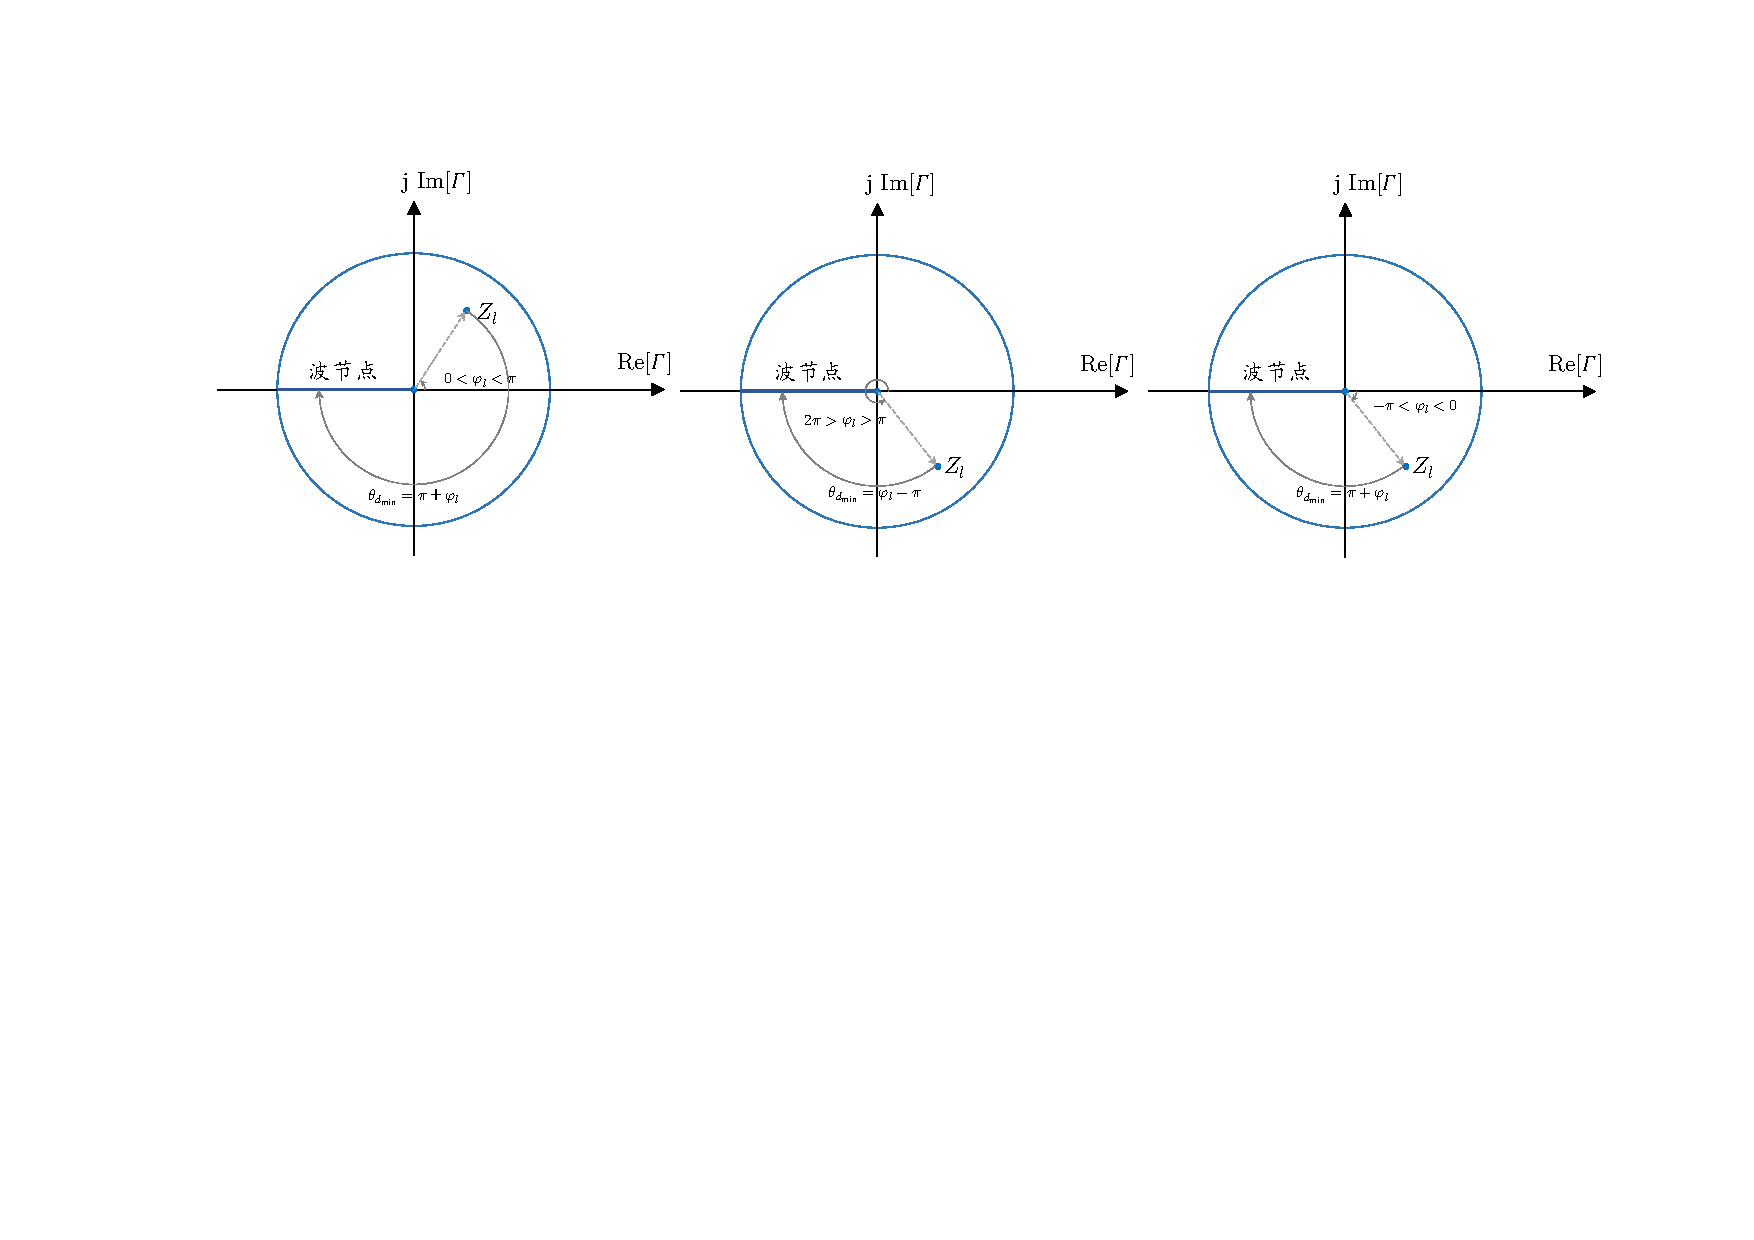
\includegraphics[width=15cm]{figure/1-2.pdf}
        \caption{\kaishu 负载到最近电压波节点的距离}\label{Fig: 负载到最近电压波节点的距离}
    \end{figure}

\section{Transmission Matrix Solution 传输矩阵解 }
\begin{center}
    \underline{约定:为了简便,本节使用的坐标系$z$为原点定义在终端,以  终端指向源端  为正方向的坐标系。}
\end{center}
因此无耗传输线模型式(\ref{Equ: Lossless Medium dudz}),(\ref{Equ: Lossless Medium didz})在当前坐标系下变为:
\begin{subequations}
    \begin{numcases}{}
        \frac{\mathrm{d}u}{\mathrm{d}z}=\mathrm{j}\omega Li \\
        \frac{\mathrm{d}i}{\mathrm{d}z}=\mathrm{j}\omega Cu
    \end{numcases}
\end{subequations}

\subsection{传输线段的矩阵解}
    \subsubsection{单边拉普拉斯变换求解无耗传输线模型}
    \begin{subequations}
        \begin{numcases}{}
            \mathscr{L}\left[\frac{\mathrm{d}u}{\mathrm{d}z}\right] \\
            d
        \end{numcases}
    \end{subequations}
    \subsubsection{传输线段矩阵}
    \subsubsection{传输线段矩阵导出输入阻抗和电压电流逆变换}
\subsection{传输矩阵的普遍理论}
    \subsubsection{传输线段的A参数矩阵}
\begin{equation}
    \begin{bmatrix}
        u_1\\i_1
    \end{bmatrix}
    =\begin{bmatrix}
        A_{11}&A_{12}\\
        A_{21}&A_{22}
    \end{bmatrix}
    \begin{bmatrix}
        u_2\\i_2
    \end{bmatrix}
\end{equation}

    \subsubsection{二端口网络性质的A参数描述}
        \begin{enumerate}
            \item 级联性质
            \begin{equation}
                \bm{A}=\prod_{i=1}^{N}\bm{A}_i
            \end{equation}
            \item 对称性质
            \begin{equation}
                A_{11}=A_{22}
            \end{equation}
            \item 无耗性质
            \begin{subequations}
                \begin{numcases}{\mbox{}}
                    A_{11},A_{22}\in\Re \\
                    A_{12},A_{21}\in\Im
                \end{numcases}
            \end{subequations}
            \item 互易性质
            \begin{equation}
                |\bm{A}|=1
            \end{equation}
            \item 阻抗变换性质
            \begin{equation}
                \begin{aligned}
                    Z_{in}&=\frac{u_1}{i_1}\\
                    &=\frac{A_{11}u_2+A_{12}i_2}{A_{21}u_2+A_{22}i_2}\\
                    &=\frac{A_{11}Z_l+A_{12}}{A_{21}Z_l+A_{22}}
                \end{aligned}
            \end{equation}
        \end{enumerate}
    
    \subsubsection{阻抗归一化的A参数矩阵}
    % 由于一个网络的端口电压和电流的关系由此处的特性阻抗所体现,因此A参数也必然和特性阻抗有关。
    此处的归一化,并非线性代数中的矩阵归一化,而是对电压波除和电流波做阻抗归一化,使其量纲变为\si{\V\per\sqrt{\Hz}}}和\si{\A\sqrt{\Hz}},然后用这种归一化阻抗的电压波和电流波定义的A参数矩阵,称之为归一化阻抗的A参数矩阵。

    将在
\subsection{微波元件的A参数矩阵}
    \subsubsection{串并联阻抗的传输矩阵}
    \subsubsection{微波传输线枝节的传输矩阵}
\section{Problems 例题讲解}
\section{Smith Chart 史密斯圆图}
\subsection{Smith圆图基本原理}
\begin{enumerate}
    \item 特征参数归一
        在史密斯圆中,阻抗和电长度要归一化。
        \begin{subequations}
            \begin{numcases}{\mbox{归一化:}}
                \bar{Z}(z')=\frac{Z(z')}{Z_0}\\
                \theta=\frac{2\pi}{\lambda_g}l
            \end{numcases}
        \end{subequations}
        \begin{equation*}
            \mbox{二次结论:}
            \begin{cases}
                \mbox{转换关系}
                \begin{cases}
                \bar{Z}(z')=\frac{1+\varGamma(z')}{1-\varGamma(z')}\\
                \varGamma(z')=\frac{\bar{Z}(z')-1}{\bar{Z}(z')+1}\\
                \end{cases}\\
                \mbox{圆基底}
                \begin{cases}
                \varGamma(z')=\left\vert \varGamma_l\right\vert \mathrm{e}^{\mathrm{j}(\varphi_l-2\beta z')}=\left\vert\varGamma_l\right\vert \mathrm{e}^{\mathrm{j}\varphi}\\
                \left\vert \varGamma(z')\right\vert=\left\vert\varGamma_l\right\vert=\left\vert\frac{\bar{Z}_l-1}{\bar{Z}_l+1}\right\vert\\
                \arg\varGamma(z')=\varphi=\varphi_l-2\beta z'=\arg\left[\frac{\bar{Z}_l-1}{\bar{Z}_l+1}\right]-2\beta z'
                \end{cases}\\
                \mbox{驻波比}\rho=\frac{1+\left\vert\varGamma_l\right\vert}{1-\left\vert\varGamma_l\right\vert}
            \end{cases}
        \end{equation*}

    \item 反射系数模值作为圆图的基底
        把反射系数沿实轴$\varGamma_r$和虚轴$\varGamma_i$分解,得到正交直角坐标系。当负载确定时,$\varGamma_l$确定,波导系统上任一点的反射系数都在以原点为圆心的圆$r=|\varGamma|$上。
        \begin{itemize}
            \item 由于反射系数模值不大于1,因此所有可能存在的$|\varGamma|$圆都在单位圆内;
        \end{itemize}


    \item 用$\left\vert \varGamma\right\vert$圆表示输入阻抗和驻波比。
        把归一化的输入阻抗$\bar{Z}$分解成电阻$r$和电抗$x$,并代入“转换关系”,可以分别解得实部和虚部满足的方程:
        \begin{subequations}
            \begin{numcases}{}
                r\mbox{满足:}\left(\varGamma_r-\frac{r}{1+r}\right)^2+\varGamma_i^2=\left(\frac{1}{1+r}\right)^2 \\
                x\mbox{满足:}\left(\varGamma_r-1\right)^2+\left(\varGamma_i-\frac{1}{x}\right)^2=\left(\frac{1}{x}\right)^2\label{Equ: 等电抗圆}
            \end{numcases}
        \end{subequations}
        它们分别对应
        \begin{itemize}
            \item 等电阻圆:圆心$\left(\frac{r}{1+r},0\right)$,半径$\frac{1}{1+r}$。与直线$\varGamma_r=1$相切于开路点;
            \item 等电抗圆:圆心$\left(1,\frac{1}{x}\right)$,半径$\frac{1}{|x|}$。与直线$\varGamma_i=0$相切于开路点;
        \end{itemize}
\end{enumerate}

\subsection{Smith圆图基本性质}
\begin{figure}[htp]
    \begin{center}
        \begin{tikzpicture}
            \begin{smithchart}[width=18cm]

                \draw (0,0) arc[start angle=180, end angle=90, radius=0.5];
                \path[->] (0,0) edge[-{Stealth[sep=3cm, bend, length=7pt, width=6pt]}, bend left=45] (0.5,0.5);
            \end{smithchart}
            % \begin{axis}[ymax=1,ymin=-1,xmax=1,xmin=-1,hide axis, height=10cm,width=10cm]
            % \addplot[color=red,mark=x] coordinates {
            % (-1,0)
            % (1,0)
            % (0,-1)
            % (0,1)
            % (0,0)
            % };
            % \end{axis}
        \end{tikzpicture}
    \end{center}
    \caption{\kaishu Smith Chart 图例}\label{Fig: Smith Chart 图例}
\end{figure}


\subsection{Smith圆图功能和应用}
\section{Impedance Matching 阻抗匹配}
\subsection{电抗性负载匹配}
    \subsubsection{网络匹配定理}
    \paragraph{无耗互易网络$\mathrm{\bm{A}}$匹配任意电抗性负载$\bar{Z}_l$的一般定理:}
    设匹配网络的A参数矩阵为$\mathrm{\bm{A}}=\begin{bmatrix}
        a_{11}&\mathrm{j}a_{12}\\
        \mathrm{j}a_{21}&a_{22}
    \end{bmatrix}$,
    则匹配时应满足振幅条件和相位条件:
    \begin{subequations}
        \begin{numcases}{\mbox{网络匹配定理}}
            \mbox{振幅条件:}\left(a_{11}-a_{22}\right)^2+\left(a_{12}-a_{21}\right)^2=\frac{4|\varGamma_l|^2}{1-|\varGamma_l|^2} \\
            \mbox{相位条件:}\begin{aligned}
                &-\arctan\left\{\frac{x_l}{r_l+1}\right\}+\arctan\left\{\frac{x_l}{r_l-1}\right\}\\
                =&\pi+\arctan\left\{\frac{a_{12}+a_{21}}{a_{11}+a_{22}}\right\}+\arctan\left\{\frac{a_{12}-a_{21}}{a_{11}-a_{22}}\right\}
            \end{aligned}
        \end{numcases}
    \end{subequations}
    此定理在后续应用单枝节匹配和双枝节匹配时并没有使用到(考的也比较少),但无论用何种方法匹配,最终的匹配网络都自动满足该定理。

\section{{\small Computation Solutions for Transmission Theory} 传输线计算机解}


\section{Problems 例题讲解}
\paragraph{1} 请写出史密斯圆图的构成思想:

消去特征参数$Z_0$(归一化),把$\beta$归于$\varGamma$相位,等$|\varGamma|$圆为基底套覆阻抗圆图和驻波比。

\paragraph{2} 如何理解史密斯圆图中“向源端为顺时针方向,向负载端为逆时针方向”?

在推导Smith圆基底——$\varGamma$的表达式的过程中,一直使用的是$z'$坐标系,它的起点是负载,正方向是源端。根据$\varGamma(z')=|\varGamma_l|\mathrm{e}^{\mathrm{j}(\varphi_l-2\beta z')}$ (\hyperref[Equ: Reflection Coefficient at z']{式(\ref*{Equ: Reflection Coefficient at z'})}),则反射系数相位随着$z'$增大而减小,因此源端方向是$\varGamma$圆的顺时针方向。

请不要把它当做结论记忆,因为有时转而使用$z$坐标系——例如设计晶体管放大器时对源端匹配条件的考虑,这时信源阻抗成了上文的负载,而晶体管的输入端成了源端,向晶体管方向是顺时针方向。

\paragraph{3} 如何快速判断史密斯圆图中的开路点和短路点?

开路点:把$Z_l=\infty$代入任一点反射系数计算公式,可得$\varGamma=1+\mathrm{j}0$。

短路点:把$Z_l=0$代入任一点反射系数计算公式,可得$\varGamma=-1+\mathrm{j}0$。

单纯地认识到“开路点在右,短路点在左”是不好的。例如在用史密斯圆图计算阻抗匹配问题时,为了得到导纳圆,将坐标轴旋转了\SI{180}{\degree},这时开路点在左边。
\paragraph{4} 如何认识史密斯圆图“上半圆表示感性,下半圆表容性”的说法?

在本节“Smith圆图基本原理”中由输入阻抗与反射系数的关系式——实部虚部对应相等求出的等电阻/电抗圆表达式可以看出,归一化电抗$x>0$,即输入阻抗呈感性则圆心在上半区域。反之位于下半区域。



最符合直觉的方法是利用任一点输入阻抗公式(\hyperref[Equ: 使用终端反射系数表示输入阻抗]{式(\ref*{Equ: 使用终端反射系数表示输入阻抗})})直接求出输入阻抗,

